\documentclass[12pt,a4paper,fleqn]{article}
\title{Progress Report}
\author{Syed Ahmad Raza}
\date{2017.03.14}
\usepackage{mathtools}
\usepackage{amsmath}
\usepackage{graphicx}
\usepackage{color}          % for color eps output
\usepackage{afterpage}
%\usepackage{layouts}       % for: \printinunitsof{in}\prntlen{\textwidth}

\begin{document}
\maketitle
\section*{Comparison of analytical and numerical solution of 2D Burgers'
equation and coding for Conjugate Gradient method}

2D form of Burgers' equation was considered, which is given mathematically as:

\begin{equation}
\frac{\partial u}{\partial t} = \frac{1}{Re}\left[\frac{\partial^2u}{\partial
x^2} + \frac{\partial^2u}{\partial y^2}\right] - u
\frac{\partial u}{\partial x} - v \frac{\partial u}{\partial y}
\end{equation}

The exact solution was carried out first and then the numerical solution was
executed using code in C++.

\begin{equation}
\frac{\partial v}{\partial t} = \frac{1}{Re}\left[\frac{\partial^2v}{\partial
x^2} + \frac{\partial^2v}{\partial y^2}\right] - u
\frac{\partial v}{\partial x} - v \frac{\partial v}{\partial y}
\end{equation}

\subsection*{Exact solution of 2D Burgers' equation}
The velocities for the exact solution are expressed as:

\begin{equation}
u = \frac{-2[a_2 + a_4y + \lambda a_5[e^{\lambda (x - x_0)} - e^{-\lambda (x -
x_0)}]\cos(\lambda y)]}{Re[a_1 + a_2x + a_3y + a_4xy + a_5[e^{\lambda (x - x_0)} + e^{-\lambda (x -
x_0)}]\cos(\lambda y)]}
\end{equation}

\begin{equation}
v = \frac{-2[a_3 + a_4x - \lambda a_5[e^{\lambda (x - x_0)} + e^{-\lambda (x -
x_0)}]\sin(\lambda y)]}{Re[a_1 + a_2x + a_3y + a_4xy + a_5[e^{\lambda (x - x_0)}
+ e^{-\lambda (x - x_0)}]\cos(\lambda y)]}
\end{equation}

where $a_1$ to $a_5$, $\lambda$ and $x_0$ provide appropriate features
to the exact solution. This equation was solved for $-1\leq x \leq 1$ and
$0 \leq y \leq \frac{\pi}{6\lambda}$. The other parameters in the steady solution
have the values $a_1 = a_2 = 1.3 \times 10^{13}, a_3 = a_4 = 0, a_5 = 1.0, \lambda = 25, x_0 =
1$ and $Re = 50$.

\subsection*{Numerical solution of Burgers' equation}
An equally spaced $50 \times 50$ grid was used to solve for the numerical
solution of the 2D Burgers' equation using code written in C++. A time step of
$10^{-6}$ was selected for the solution. Dirichlet boundary conditions using the
exact solution were chosen and initial conditions of $u_i = 0.1$ and $v_i = 0.0$
were selected for testing purposes (regardless of the physicality of the flow).

Central difference scheme was used for the solution, as given by the following
formula:

\begin{equation}
\begin{split}
u_{i,j}^{n+1}=\quad &u_{i,j}^n + \Delta t
\bigg[\frac{1}{Re}\left(\frac{u_{i,j+1}^n - 2u_{i,j}^n + u_{i,j-1}^n}{(\Delta
x)^2} + \frac{u_{i+1,j}^n - 2u_{i,j}^n + u_{i-1,j}^n}{(\Delta y)^2}\right)
\\&- u_i^n\left(\frac{u_{i,j+1}^n - u_{i,j-1}^n}{2\Delta x}\right) -
v_i^n\left(\frac{u_{i+1,j}^n - u_{i-1,j}^n}{2\Delta y} \right) \bigg]
\end{split}
\end{equation}

\begin{equation}
\begin{split}
v_{i,j}^{n+1}=\quad &v_{i,j}^n + \Delta t
\bigg[\frac{1}{Re}\left(\frac{v_{i,j+1}^n - 2v_{i,j}^n + v_{i,j-1}^n}{(\Delta
x)^2} + \frac{v_{i+1,j}^n - 2v_{i,j}^n + v_{i-1,j}^n}{(\Delta y)^2}\right)
\\&- v_i^n\left(\frac{v_{i,j+1}^n - v_{i,j-1}^n}{2\Delta x}\right) -
v_i^n\left(\frac{v_{i+1,j}^n - v_{i-1,j}^n}{2\Delta y} \right) \bigg]
\end{split}
\end{equation}

\begin{figure}[p!]
\centering
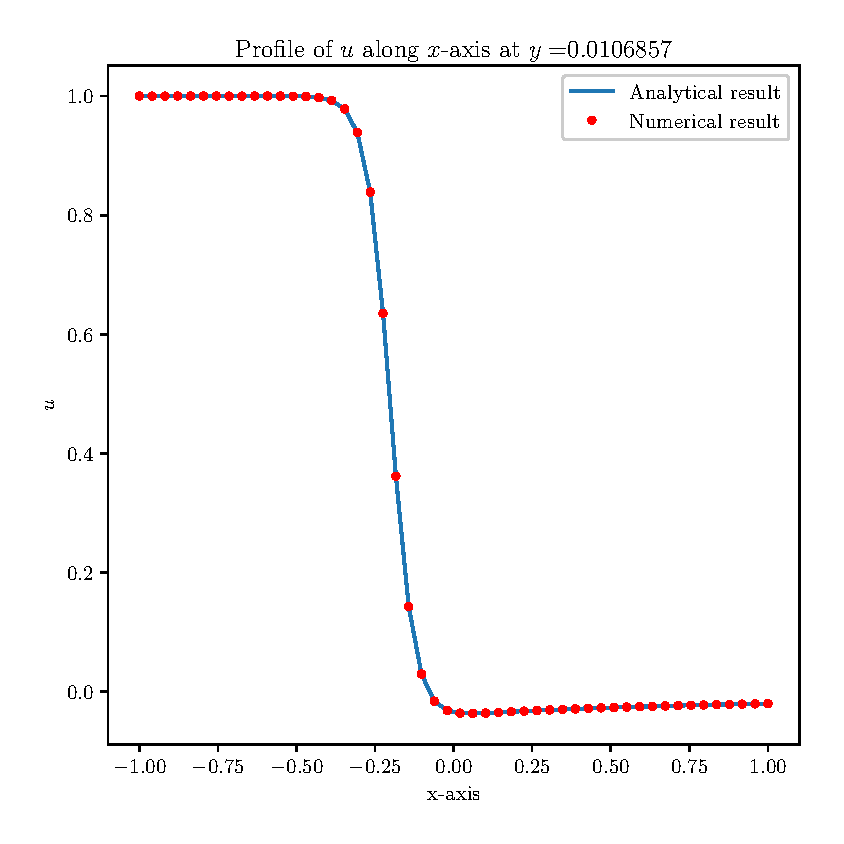
\includegraphics[width=\linewidth]{comparisonU.eps}
\caption{Comparison of numerical solution and exact solution of the 2D Burgers'
equation for velocity component $u$.}
\end{figure}


\begin{figure}[p!]
\centering
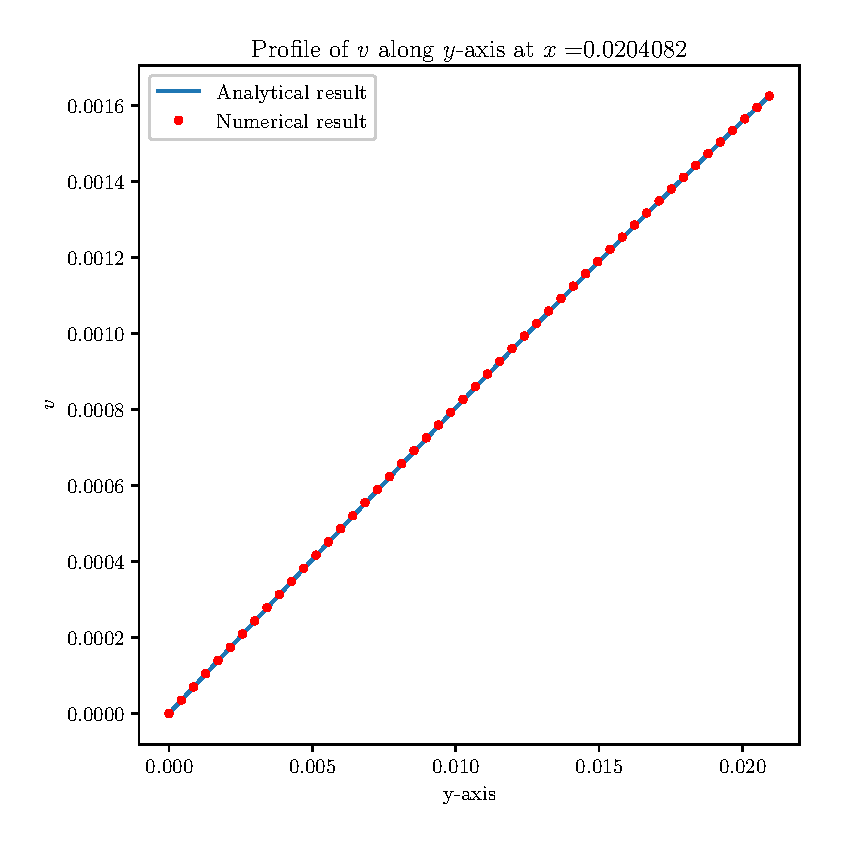
\includegraphics[width=\linewidth]{comparisonV.eps}
\caption{Comparison of numerical solution and exact solution of the 2D Burgers'
equation for velocity component $v$.}
\end{figure}

\newpage

\subsection*{Solving a system of equations using Conjugate Gradient method}

A code has been developed in C++ to solve the following set of equations using
Conjugate Gradient method:

\begin{equation}
4x_1 + x_2 = 1
\end{equation}
\begin{equation}
x_1 + 3x_2 = 2
\end{equation}

The true solution is $x_1
= 0.0909$ and $x_2 = 0.6364$, which was achieved after 2 iterations.

\end{document}